\documentclass[useAMS,usenatbib,referee]{enar}

\newtheorem{thm}{Theorem}[section] \newtheorem{deff}[thm]{Definition}
\newtheorem{rmk}[thm]{Remark} \newtheorem{prf}[thm]{Proof}
\newtheorem{cor}[thm]{Corollary} \newtheorem{emp}[thm]{Example}
\newtheorem{lem}[thm]{Lemma} \newtheorem{pps}[thm]{Proposition}
\newcommand{\iid}{\stackrel{\mbox{i.i.d}}{\sim}}
\newcommand{\pr}{\mbox{p}}
\newcommand{\prob}{\mbox{Pr}}
\newcommand{\polya}{P\'{o}lya} \newcommand{\yobs}{\bmath y_{\itl{obs}}}
\newcommand{\ymis}{\bmath y_{\itl{mis}}}

\usepackage[figuresright]{rotating}

\usepackage{amsmath}

\title[ ]{Quantile Regression in the Presence of Monotone Missingness with Sensitivity Analysis}

\begin{document}

\label{firstpage}

\begin{abstract}
  In this paper, we develop methods for longitudinal quantile
  regression when there is monotone missingness. In particular, we
  propose pattern mixture models with a constraint that provides an
  interpretation form for the marginal quantile regression
  parameters. Our approach allows sensitivity analysis and informative
  priors which are an essential component in inference for incomplete
  data. To facilitate computation of the likelihood, we propose a
  novel way to obtain analytic forms for integrals in likelihood. Both
  frequentist and Bayesian inferences are illustrated. The model is
  applied to data from a clinical trial on weight management.
\end{abstract}

\begin{keywords}
  Monotone missingness; Non-ignorable missingness; Quantile regression;
  Sensitivity analysis.
\end{keywords}

\maketitle

\section{Introduction}

Quantile regression is used to study the relationship between a
response and covariates when one (or several) quantiles are of
interest as opposed to mean regression.  The dependence between upper
or lower quantiles of the response variable and the covariates often
vary differentially relative to that of the mean. How quantiles depend
on covariates is of interest in econometrics, educational studies,
biomedical studies, and environment studies \citep{yu2001,
  buchinsky1994,buchinsky1998,he1998, koenker1999,wei2006,yu2003}. A
comprehensive review of applications of quantile regression was
presented in \citet{koenker2005}.

Quantile regression is more robust to outliers than mean regression
and provides information about how covariates affect quantiles, which
offers a more complete description of the conditional distribution of
the response. Different effects of covariates can be assumed for
different quantiles.

The traditional frequentist approach was proposed by
\citet{koenker1978} for a single quantile with estimators derived by
minimizing a loss function. The popularity of this approach is due to
its computational efficiency, well-developed asymptotic properties,
and straightforward extensions to simultaneous quantile regression and
random effect models. However, asymptotic inference may not be
accurate for small sample sizes and the approach does not naturally
extend to missing data.

Bayesian approaches offer exact inference in small samples. Motivated
by the loss (check) function, \citet{yu2001} proposed an asymmetric
Laplace distribution for the error term, such that maximizing the
posterior distribution is equivalent to minimizing the check function.
Also semiparametric methods have been proposed for median
regression. \citet{walker1999} used a diffuse finite \polya{} Tree
prior for the error term. \citet{kottas2001} modeled the error by two
families of median zero distribution using a mixture Dirichlet process
priors, which is very useful for unimodal error
distributions. \citet{hanson2002} adopted mixture of \polya{} Tree
prior in median regression, which is more robust in terms of
multimodality and skewness. Other recent approaches include quantile
pyramid priors, mixture of Dirichlet process priors of multivariate
normal distributions and infinite mixture of Gaussian densities which
place quantile constraints on the residuals \citep{hjort2007,
  hjort2009, kottas2009,reich2010}.

The above methods focus on complete data.  There are only a few
articles about quantile regression with missingness.  \citet{wei2012}
proposed a multiple imputation method for quantile regression model
when there are some covariates missing at random (MAR). They impute
the missing covariates by specifying its conditional density given
observed covariates and outcomes, which come from the estimated
conditional quantile regression and specification of conditional
density of missing covariates given observed ones.  However, they put
more focus on the missing covariates rather than missing outcomes.
\citet{bottai2013} illustrated an imputation method using estimated
conditional quantiles of missing outcomes given observed data. Their
approach does not make distributional assumptions.  They assumed the
missing data mechanism (MDM) is ignorable. However, because their
imputation method is not derived from a joint distribution, the joint
distribution with such conditionals may not exist.  In addition, their
approach does not allow for MNAR.

\citet{yuan2010} introduced a fully parametric Bayesian quantile
regression approach for longitudinal data with non-ignorable missing
data. They used shared latent subject-specific random effects to
explain the within-subject correlation and to associate the response
process with missing data process, and applied multivariate normal
priors on the random terms to match the traditional quantile
regression check function with penalties. However, the quantile
regression coefficients are conditional on the random effects, which
is not of interest if we are interested in interpreting regression
coefficients unconditionally.  In addition, they are
conditional on random effects, which tie together the responses and
missingness process, so they have slightly different interpretation
than regular random effects in longitudinal methods. Moreover, due to
their full parametric specification for the full data, their model
does not allow for sensitivity analysis, which is a key component in
inference for incomplete data (NAS 2010).

Pattern mixture models were originally proposed to model missing data
in \citet{rubin1977}. Later mixture models were extended to handle
MNAR in longitudinal data. For discrete dropout times,
\citet{little1993, little1994} proposed a general method by
introducing a finite mixture of multivariate distribution for
longitudinal data. When there are many possible dropout time,
\citet{roy2003} proposed to group them by latent classes.

\citet{roy2008} extended \citet{roy2003} to generalized linear models
and proposed a pattern mixture model for data with non-ignorable
dropout, borrowing ideas from \citet{heagerty1999}.  But their
approach only estimates the marginal covariate effects on the mean. We
will use related ideas for quantile regression models which allows for
non-ignorable missingness and sensitivity analysis.

The structure of this article is as follows. First, we introduce a
quantile regression method to address monotone non-ignorable
missingness in section \ref{sec:model}, including sensitivity analysis
and computational details.  We use simulation studies to evaluate the
performance of the model in section \ref{sec:simulation}. We apply our
approach to data from a recent clinical trial in section
\ref{sec:real}. Finally, discussion and conclusions are given in
section \ref{sec:discussion}.

\section{Model}
\label{sec:model}

In this section, we first introduce some notation, then describe our
proposed quantile regression model in section \ref{sec:settings}. We
provide details on MAR and MNAR and computation in sections
\ref{sec:sa} and \ref{sec:computation} respectively.

Under monotone dropout, without loss of generality, denote $S_i \in
\{1, 2, \ldots, J\}$ to be the number of observed $Y_{ij}'s$ for
subject $i$, and $\bmath Y_i = (Y_{i1}, Y_{i2}, \ldots, Y_{iJ})^{T}$ to
be the full data response vector for subject $i$, where $J$ is the
maximum follow up time. We assume $Y_{i1}$ is always observed. We are
interested in the $\tau$-th marginal quantile regression coefficients
$\bmath \gamma_j = (\gamma_{j1}, \gamma_{j2}, \ldots, \gamma_{jp})^T$,
\begin{equation}\label{eq:marg}
  \prob (Y_{ij} \leq \bmath x_i^{T} \bmath \gamma_j ) = \tau, \mbox{ for } j = 1, \ldots, J,
\end{equation}
where $\bmath x_i$ is a $p \times 1$ vector of covariates for subject
$i$.

Let
\begin{displaymath}
  \pr_k(Y) = \pr (Y | S = k), \quad  \pr_{\geq k} (Y)  = \pr (Y | S \geq k)
\end{displaymath}
be the densities of response $\bmath Y$ given follow-up time $S=k$ and $S
\geq k$. And $\prob_k$ be the corresponding probability given $S = k$.

\subsection{Mixture Model Specification}
\label{sec:settings}
We adopt a pattern mixture model to jointly model the response and
missingness \citep{little1994, dh2008}. Mixture models factor the
joint distribution of response and missingness as
\begin{displaymath}
  \pr (\bmath y, \bmath S, |\bmath x, \bmath \omega) = \pr (\bmath y|\bmath S, \bmath x, \bmath \omega) \pr (\bmath S | \bmath x, \bmath \omega).
\end{displaymath}
Thus the full-data response follows the distribution given by
\begin{displaymath}
  \pr (\bmath y | \bmath x, \bmath \omega) = \sum_{S \in \mathcal{S}} \pr(\bmath y| \bmath S, \bmath x, \bmath \theta) \pr (\bmath S | \bmath x, \bmath \phi),
\end{displaymath}
where $\mathcal{S}$ is the sample space for dropout time $S$ and the
parameter vector $\bmath \omega$ is partitioned as $(\bmath \theta, \bmath
\phi)$.

Furthermore, the conditional distribution of response within patterns
can be decomposed as
\begin{equation}\label{eq:decompose}
  \pr (\yobs, \ymis | \bmath S, \bmath \theta) = \pr
  (\ymis|\yobs, \bmath S, \bmath \theta_E) \pr (\yobs | \bmath S, \bmath
  \theta_{y, O}),
\end{equation}
where $\bmath \theta_E$ indexes the parameters in the extrapolation
distribution, the first term on the right hand side and $\bmath
\theta_{y, O}$ indexes parameters in the distribution of observed
responses, the second term on the right hand side.

We assume models within pattern to be multivariate normal
distributions and specify a sequential model parametrization.
First we specify the marginal
quantile regression models from equation \eqref{eq:marg}.

Then we specify the conditional distributions on $S$ as:
\begin{equation}
  \begin{array}{l}
      \displaystyle \pr_k(y_{i1}) = N (\Delta_{i1} + \bmath x_{i1}^T \bmath \beta_1^{(k)},
      \sigma_1^{(k)}  ), k = 1, \ldots, J,\\
       \displaystyle \pr_k(y_{ij}|\bmath y_{ij^{-}}) =
      \begin{cases}
        \textrm{N} \big (\Delta_{ij} + \bmath x_{ij}^T \bmath h_{j}^{(k)} +
        \bmath y_{ij^{-}}^T \bmath \beta_{y,j-1}^{(k)},
        \sigma_j^{(k)} \big), & k < j ;  \\
        \textrm{N} \big (\Delta_{ij} + \bmath y_{ij^{-}}^T \bmath
        \beta_{y,j-1}^{(\geq j)},
        \sigma_j^{(\geq j)} \big), & k \geq j ;  \\
      \end{cases}, \mbox{ for } 2 \leq j \leq J,  \\
      \displaystyle S_{ij} = k| \bmath x_{ij} \sim \textrm{Multinomial}(1, \bmath \phi),
    \end{array}
  \label{eq:model}
\end{equation}
where $\bmath y_{ij^{-}} = (y_{i1}, \ldots, y_{i(j-1)})^T$ is the
response history for subject $i$ up to time point  $(j-1)$; $\bmath \phi =
(\phi_1, \ldots, \phi_J)$ is the multinomial probability vector for the
number of observed responses; $\bmath h_j^{(k)} = (h_{j1}^{(k)}, \ldots,
h_{jp}^{(k)})$ are sensitivity parameters which we will discuss in
section \ref{sec:sa}.  $\bmath x_{ij}$ is a $p \times 1$ covariate vector;
$\bmath \beta_{y, j-1}^{(k)} = \big(\beta_{y_1, j-1}^{(k)}, \ldots,
\beta_{y_{j-1}, j-1}^{(k)} \big)^T$ are autoregressive coefficients
and $\sigma_j^{(k)}$ is the conditional standard deviation of response
component $j$. We specify the model as in (\ref{eq:model}) to have
multivariate normal distribution within patterns such that MAR exists
\citep{wang2011}. More details are presented in section \ref{sec:sa}.

In (\ref{eq:model}), $\Delta_{ij}$ are functions of $\tau, \bmath x_{ij},
\bmath \beta, \bmath h, \bmath \sigma, \bmath \gamma_j, \bmath \phi$ and are determined by the marginal
quantile regressions,
\begin{equation}
  \label{eq:deltaeqn1}
  \tau = \prob (Y_{ij} \leq \bmath x_{ij}^T \bmath \gamma_j ) = \sum_{k=1}^J
  \phi_k\prob_k (Y_{ij} \leq \bmath x_{ij}^T \bmath \gamma_j ) \mbox{  for  } j = 1,
\end{equation}
and
\begin{align}\label{eq:deltaeqn2}
  \tau &= \prob (Y_{ij} \leq \bmath x_{ij}^{T} \bmath \gamma_j ) =
  \sum_{k=1}^J
  \phi_k\prob_k (Y_{ij} \leq \bmath x_{ij}^{T} \bmath \gamma_j ) \\
  & = \sum_{k=1}^J \phi_k \int\cdots \int \prob_k (Y_{ij} \leq \bmath
  x_{ij}^{T} \bmath \gamma_j | \bmath y_{ij^{-}}
  ) \pr_k (y_{i(j-1)}| \bmath y_{i(j-1)^{-}})  \nonumber \\
  & \quad \cdots \pr_k (y_{i2}| y_{i1}) \pr_k(y_{i1})
  dy_{i(j-1)}\cdots dy_{i1}.  \mbox{  for  } j = 2, \ldots, J .\nonumber
\end{align}
Computational details will be given in section
\ref{sec:computation}.

The idea is to model the marginal quantile regressions directly, then
to embed them in the likelihood through restrictions in the mixture
model. The mixture model in (\ref{eq:model}) allows the marginal
quantile regression coefficients to differ by quantiles. Otherwise,
the quantile lines would be parallel to each other. Moreover, the
mixture model also allows sensitivity analysis.

For identifiability of the observed data distribution, we apply the
following restrictions,
\begin{displaymath}
 \sum_{k=1}^J \beta_{l1}^{(k)} = 0, l = 1,\ldots, p,
\end{displaymath}

\subsection{Missing Data Mechanism and Sensitivity Analysis}
\label{sec:sa}

In general, mixture models are not identified due to insufficient
information provided by observed data. Specific forms of missingness
are needed to induce constraints to identify the distributions for
incomplete patterns, in particular, the extrapolation distribution in
(\ref{eq:decompose}). In this section, we explore ways to embed the
missingness mechanism and sensitivity parameters in mixture models for
our setting.

In the mixture model in (\ref{eq:model}), MAR holds \citep{molen1998,
  wang2011} if and only if, for each $j \geq 2$ and $k < j$:
\begin{displaymath}
  \pr_k(y_j|y_1, \ldots, y_{j-1}) = \pr_{\geq j}(y_j|y_1, \ldots, y_{j-1}).
\end{displaymath}
When $2 \leq j \leq J$ and $k < j$, $Y_j$ is not observed, thus
$\bmath h_j^{(k)}$ and $ \sigma_j^{(k)}$, $ \bmath \beta_{y,
  j-1}^{(k)} = \big(\beta_{y_1,j}^{(k)}, \ldots,
\beta_{y_{j-1},j-1}^{(k)} \big)^T $ can not be identified from the
observed data. Denote
\begin{align*}
  \log \sigma_j^{(k)} &= \log \sigma_j^{(\geq j)} +  \delta_{j}^{(k)}, \\
  \bmath \beta_{y, j-1}^{(k)} &= \bmath \beta_{y, j-1}^{(\geq j)} +
  \bmath \eta_{j-1}^{(k)},
\end{align*}
where $\bmath \eta_{j-1}^{(k)} = \big( \eta_{y_1,j-1}^{(k)}, \ldots,
\eta_{y_{j-1}, j-1}^{(k)} \big)$ for $k < j$. Then $\bmath \xi_s = (
\bmath h_j^{(k)}, \bmath \eta_{j-1}^{(k)}, \delta_j^{(k)})$ is a set
of sensitivity parameters \citep{dh2008}, where $k < j, 2 \leq j \leq
J $.

When $\bmath \xi_s = \bmath \xi_{s0} = \bmath 0$, MAR holds. If
$\bmath \xi_s$ is fixed at $\bmath \xi_s \neq \bmath \xi_{s0}$, the
missingness mechanism is MNAR. We can vary $\bmath \xi_s$ around
$\bmath 0$ to examine the impact of different MNAR mechanisms.

For fully Bayesian inference, we can put priors on $(\bmath \xi_s,
\bmath \xi_m)$ as :
\begin{displaymath}
  p(\bmath \xi_s, \bmath \xi_m) = p(\bmath \xi_s) p(\bmath \xi_m),
\end{displaymath}
where $\bmath \xi_m = \big(\bmath \gamma_j, \bmath \beta_{y,
  j-1}^{(\geq j)}, \bmath \alpha_j^{(\geq j)}, \bmath \phi \big)$, the
identified parameters in the data distribution.  If we assume MAR with
no uncertainty, the prior of $\bmath \xi_s$ is $\pr(\bmath \xi_s =
\bmath 0) \equiv 1$. Sensitivity analysis can be executed by putting
point mass priors on $\bmath \xi_s$ to examine the effect of priors on
the posterior inference about quantile regression coefficients $\bmath
\gamma_{j}^{\tau}$. For example, if MAR is assumed with uncertainty,
priors can be assigned as $\textrm{E}(\bmath \xi_s) = \bmath \xi_{s0}
= \bmath 0$ with $\textrm{Var}(\bmath \xi_s) \neq \bmath 0$. If we
assume MNAR with no uncertainty, we can put priors satisfying
$\textrm{E}(\bmath \xi_s) = \Delta_{\xi}$, where $\Delta_{\xi} \neq
\bmath 0$ and $\textrm{Var}(\bmath \xi_s) = \bmath 0$. If MNAR is
assumed with uncertainty, then priors could be $\textrm{E}(\bmath
\xi_s) = \Delta_{\xi}$, where $\Delta_{\xi} \neq \bmath 0 $ and
$\textrm{Var}(\bmath \xi_s) \neq \bmath 0$.

In general, each pattern $S = k$ has its own set of sensitivity
parameters $\bmath \xi_s^{(k)}$. However, to keep the number of
sensitivity parameters at a manageable level \citep{dh2008} and
without loss of generality, we assume $\bmath \xi_s$ does not depend
on pattern.

\subsection{Computation}
\label{sec:computation}

In section \ref{sec:deltacal}, we provide details on calculating
$\Delta_{ij}$ in (\ref{eq:model}) for $j = 1, \ldots, J$. Then we show
how to obtain maximum likelihood estimates in section
\ref{sec:mle}. Finally, we present a Monte Carlo Markov Chain (MCMC)
sampling algorithm for Bayesian inference in section
\ref{sec:bayesian}.

\subsubsection{Calculation of $\Delta$ }
\label{sec:deltacal}
From equation (\ref{eq:deltaeqn1}) and (\ref{eq:deltaeqn2}),
$\Delta_{ij}$ depends on subject-specific covariates $\bmath x_{ij}$,
thus $\Delta_{ij}$ needs to be calculated for each subject. We now
illustrate how to calculate $\Delta_{ij}$ given all the other
parameters $\bmath \xi = (\bmath \xi_m, \xi_s)$.

\begin{itemize}
\item \textbf{$\Delta_{i1}: $} Expand equation (\ref{eq:deltaeqn1}):
  \begin{align*}
    \tau = \sum_{k = 1}^J \phi_k \Phi \left( \frac{\bmath x_{i1}^T
        \bmath \gamma_1 - \Delta_{i1} - \bmath x_{i1}^T\bmath
        \beta_1^{(k)}}{ \sigma_1^{(k)} } \right),
  \end{align*}
  where $\Phi$ is the standard normal CDF. Because the above equation
  is continuous and monotone in $\Delta_{i1}$, it can be solved by a
  standard numerical root-finding method (e.g. bisection method) with
  minimal difficulty.

\item \textbf{$\Delta_{ij}, 2\leq j \leq J: $}

  First we introduce a lemma:
  \begin{lem}\label{sec:lemma}
    An integral of a normal CDF with mean $b$ and standard deviation
    $a$ over another normal distribution with mean $\mu$ and standard
    deviation $\sigma$ can be simplified to a closed form in terms of
    normal CDF:
    \begin{displaymath}
      \int \Phi \left( \frac{x-b}{a} \right) d\Phi(x; \mu, \sigma)  =
      \begin{cases}
        1- \Phi \left( \frac{b-\mu}{\sigma} \big /
          \sqrt{\frac{a^2}{\sigma^2}+1} \right) & a > 0, \\
        \Phi \left( \frac{b-\mu}{\sigma} \big /
          \sqrt{\frac{a^2}{\sigma^2}+1} \right) & a < 0,
      \end{cases}
    \end{displaymath}
    where $\Phi(x; \mu, \sigma)$ stands for a CDF of normal
    distribution with mean $\mu$ and standard deviation $\sigma$.
  \end{lem}

  Given the result in Lemma \ref{sec:lemma}, to solve equation
  (\ref{eq:deltaeqn2}), we propose a recursive approach. For the first
  multiple integral in equation (\ref{eq:deltaeqn2}), apply lemma
  \ref{sec:lemma} once to obtain:
  \begin{align*}
    \prob_1 (Y_{ij} \leq \bmath x_{ij}^T \bmath \gamma_j) & =
    \int\dots\int
    \prob (Y_{ij} \leq \bmath x_{ij}^T\bmath \gamma_j | S=1, \bmath x_{ij}, \bmath Y_{ij^{-}})\\
    & \quad  dF(Y_{i(j-1)}|S=1, \bmath x_{ij}, \bmath Y_{i(j-1)^{-}}) \cdots d F (Y_{i1} | S = 1, \bmath x_{ij}), \\
    & = \int\dots\int
    \Phi \left( \frac{\bmath x^T \bmath \gamma_j - \mu_{j|1, \ldots, j-1}(\bmath Y_{ij^{-}})}{\sigma_{j|1, \ldots, j-1}} \right) \\
    & \quad   dF(Y_{i(j-1)}|S=1, \bmath x_{ij}, \bmath Y_{i(j-1)^{-}}) \cdots d F (Y_{i1} | S = 1, \bmath x_{ij}), \\
    & = \int\dots\int \Phi \left( \frac{Y_{i(j-2)} - b^{*}}{a^{*}}
    \right) dF(Y_{i(j-2)}|S=1, \bmath x_{ij}, \bmath Y_{i(j-2)^{-}}) \\
    & \quad \cdots d F (Y_{i1} | S = 1, \bmath x_{ij}).
  \end{align*}

  Then, by recursively applying lemma \ref{sec:lemma} $(j-1)$ times,
  each multiple integral in equation (\ref{eq:deltaeqn2}) can be
  simplified to single normal CDF. Thus we can easily solve for
  $\Delta_{ij}$ using standard numerical root-finding method as for $j
  = 1$.

\end{itemize}

\subsubsection{Maximum Likelihood Estimation}
\label{sec:mle}

The observed data likelihood for an individual $i$ with follow-up time
$S_i = k$ is
\begin{align} \label{eq:ll} L_i(\bmath \xi| \bmath y_i, S_{i} = k) & =
  \phi_k\pr_k (y_k | y_1, \ldots, y_{k-1})
  \pr_k (y_{k-1}|y_1, \ldots, y_{k-2}) \cdots \pr_{k} (y_1), \\
  & = \phi_k \pr_{\geq k} (y_k | y_1, \ldots, y_{k-1}) \pr_{\geq k-1}
  (y_{k-1}|y_1, \ldots, y_{k-2}) \cdots \pr_{k} (y_1), \nonumber
\end{align}
where $\bmath y_i = (y_1, \ldots, y_k)$.

We use derivative-free optimization algorithms by quadratic
approximation to compute the maximum likelihood estimates
\citep{minqa}. Denote $J(\bmath \xi) = - \log L = - \log \sum_{i =
  1}^n L_i$.  Then maximizing the likelihood is equivalent to minimizing
the target function $J(\bmath \xi)$. Under an MAR assumption, we fix
$\bmath \xi_s = \bmath 0$, while under MNAR assumption, $\bmath \xi_s
$ can be chosen as desired.

During each step of the algorithm, $\Delta_{ij}$ has to be calculated
for each subject and at each time, as well as partial derivatives for
each parameter.

As an example of the speed of the algorithm, for 100 bivariate
outcomes and 5 covariates, it takes about 1.9 seconds to get
convergence using R version 2.15.3 (2013-03-01) \citep{R} and
platform: x86\_64-apple-darwin9.8.0/x86\_64 (64-bit). Main parts of
the algorithm are coded in Fortran such as calculation of numerical
derivatives and log-likelihood to quicken computations. We have
incorporated those functions implementing the algorithm into the new R
\citep{R} package ``qrmissing''.

We use the bootstrap \citep{efron1979,efron1993,divison1997} to
construct confidence interval and make inferences.  We resample
subjects and use bootstrap percentile intervals to form confidence
intervals.

\subsubsection{Goodness of Fit Check}
\label{sec:goodness}
A simple goodness-of-fit check can be done by examining normal QQ
plots of the fitted residuals from the model. The visual test can help
to diagnose if the parametric assumptions are suitable for model.

After obtaining the MLE, we use the approach described in section
\ref{sec:deltacal} to get the fitted $\Delta_{ij}$ for each
subject. Then the fitted residuals can be obtained by plugging in the
fitted estimates and $\hat{\Delta}_{ij}$ to obtain,
\begin{displaymath}
  \hat{\epsilon}_{ij} =
  \begin{cases}
    (y_{ij} - \hat{\Delta}_{ij} - \bmath{x_{ij}^T
    \hat{\beta}_1^{(k)}})/\hat{\sigma}_1^{(k)},& j = 1 \\
    (y_{ij} - \hat{\Delta}_{ij} - \bmath{y_{ij^{-}}^T
    \hat{\beta}_{y,j-1}^{(\geq j)}})/\hat{\sigma}_j^{(\geq j)},& j >
    1
  \end{cases}.
\end{displaymath}

\subsubsection{Bayesian Framework}
\label{sec:bayesian}

For Bayesian inference, we specify priors on the parameters $\bmath
\xi$ and use a block Gibbs sampling method to draw samples from the
posterior distribution. Denote all the parameters to sample as :
\begin{align*}
  \bmath \xi_m &= \left\{ \bmath \gamma_j,
    \bmath \beta_{y,j-1}^{(\geq j)}, \bmath \alpha_j^{(\geq j)} \right\}
  \mbox{ for } j = 1, \ldots, J ,\\
  \bmath \xi_s &= \left\{ \bmath h_j^{(k)}, \bmath \eta_{j-1}^{(k)},  \delta_j^{(k)}
  \right\}
  \mbox{ for } k = 1, \ldots, j-1; 2 \leq j \leq J.
\end{align*}
Comma separated parameters are marked to sample as a block.  Updates
of $\bmath \xi_m$ require a Metropolis-Hasting algorithm, while
$\bmath \xi_s$ samples are drawn directly from priors as desired for
missingness mechanism assumptions.

As mentioned in section \ref{sec:sa}, MAR or MNAR assumptions are
implemented via specific priors. For example, if MAR is assumed with
no uncertainty, then $ \bmath \xi _s= \bmath 0$ with probability
1. Details for updating parameters are:

\begin{itemize}
\item $\bmath \gamma_{1} $: Use Metropolis-Hasting algorithm.
  \begin{enumerate}
  \item Draw ($\bmath \gamma_{1}^c$) candidates from candidate
    distribution;
  \item Based on the new candidate parameter $\bmath \gamma^c$, calculate
    candidate $\Delta_{ij}^c$ for each subject $i$ as we described in
    section \ref{sec:deltacal}.
  \item Plug in $\Delta_{ij}^c$ in likelihood (\ref{eq:ll}) to get
    candidate likelihood;
  \item Compute Metropolis-Hasting ratio, and accept the candidate
    value or keep the previous value.
  \end{enumerate}
\item For the rest of the identifiable parameters, algorithms for
  updating the samples are all similar to $\bmath \gamma_j$.
\item For sensitivity parameters, because we do not get any
  information from the data, we sample them from priors, which are
  specified based on assumptions about the missingness.
\end{itemize}

\section{Simulation Study}
\label{sec:simulation}
In this section, we compare the performance of our proposed model in
section \ref{sec:settings} with the \textit{rq} function (noted as RQ) in
\textit{quantreg} R package \citep{quantreg} and Bottai's algorithm
\citep{bottai2013} (noted as BZ). The \textit{rq} function
minimizes the loss (check) function $\sum_{i=1}^n \rho_{\tau} (y_i -
\bmath x_i^T \bmath \beta)$ in terms of $\bmath \beta$, where the loss
function $\rho_{\tau} (u) = u(\tau - I(u < 0))$ and does not make any
distributional assumptions. \citet{bottai2013} impute missing
outcomes using the estimated conditional quantiles of missing outcomes
given observed data. Their approach does not make distributional
assumptions similar to \textit{rq} and assumes MAR missing data.

We considered three scenarios corresponding to both MAR and MNAR
assumptions for a bivariate response.  In the first scenario, $Y_2$
were missing at random and we used the MAR assumption in our
algorithm. In the next two scenarios, $Y_2$ were missing not at
random. However, in the second scenario, we misspecified the MDM for
our algorithm and still assumed MAR, while in the third scenario, we
used the correct MNAR MDM. For each scenario, we considered three
error distributions: normal, student t distribution with 3 degrees of
freedom and Laplace distribution. For each error model, we simulated
100 data sets. For each set there are 200 bivariate observations
$\bmath Y_i = (Y_{i1}, Y_{i2})$ for $i = 1, \ldots, 200$. $Y_{i1}$
were always observed, while some of $Y_{i2}$ were missing. A single
covariate $x$ was sampled from Uniform(0,2). The three models for the
full data response $\bmath Y_i$ were:
\begin{align*}
  Y_{i1} | R = 1 & \sim 2 + x_i +  \epsilon_{i1} , \\
  Y_{i1}| R = 0 & \sim  -2 - x_i +  \epsilon_{i1} , \\
  Y_{i2}| R = 1, Y_{i1}&\sim 1 - x_i - 1/2Y_{i1} + \epsilon_{i2},
\end{align*}
where $\epsilon_{i1}, \epsilon_{i2} \iid \textrm{N}(0, 1)$, $t_3$ or
$\mbox{LP}(\mbox{rate} = 1)$ distribution within each scenario.

For all cases, $\prob (R = 1) = 0.5$.  When $R = 0$, $Y_{i2}$ is not
observed, so $\pr(Y_{i2}| R = 0, Y_{i1})$ is not identifiable from
observed data.

In the first scenario, $Y_2$ is missing at random, thus $\pr(Y_{i2} |
R = 0, Y_{i1}) = \pr(Y_{i2}|R = 1, Y_{i1}) $. In the last two
scenarios, $Y_2$ are missing not at random. We assume $Y_{i2}| R = 0,
Y_{i1} \sim 3 - x_i - 1/2Y_{i1} + \epsilon_{i2}$. Therefore, there is
a shift of 2 in the intercept between $\pr(Y_2|R = 1, Y_1)$ and
$\pr(Y_2|R = 0, Y_1)$.

Under an MAR assumption, the sensitivity parameter $\bmath \xi_s$ is
fixed at $\bmath 0$ as discussed in section \ref{sec:sa}. For
\textit{rq} function from \textit{quantreg} R package, because only
$Y_{i2}|R = 1$ is observed, the quantile regression for $Y_{i2}$ can
only be fit from the information of $Y_{i2}|R = 1$ vs $x$.

In scenario 2 under MNAR, we mis-specified the MDM using the wrong
sensitivity parameter $\bmath \xi_s$ at $\bmath 0$. In scenario 3, we
assumed there was an intercept shift between distribution of
$Y_{i2}|Y_{i1}, R = 1$ and $Y_{i2}|Y_{i1}$, $R = 0$, thus fixed
$\bmath \xi_s$ at its true value.

For each dataset, we fit quantile regression for quantiles $\tau =$
0.1, 0.3, 0.5, 0.7, 0.9.  Parameter estimates were evaluated by mean
squared error (MSE),
\begin{displaymath}
  \mbox{MSE} (\gamma_{ij}) = \frac{1}{100} \sum_{k = 1}^{100}
  \left( \hat{\gamma}_{ij}^{(k)}  - \gamma_{ij}\right)^2, i = 0, 1
\end{displaymath}
where $\gamma_{j}$ is the true value for quantile regression
coefficient, $\hat{\gamma}_{j}^{(k)}$ is the maximum likelihood
estimates in $k$-th simulated dataset ($(\gamma_{01}, \gamma_{11})$
for $Y_{i1}$, $(\gamma_{02}, \gamma_{12})$ for $Y_{i2}$).

Monte Carlo standard error (MCSE) is used to evaluate the significance
of difference between methods. It is calculated by
\begin{displaymath}
  \mbox{MCSE} = \hat{\mbox{sd}}(\mbox{Bias}^2)/\sqrt{N},
\end{displaymath}
where $\hat{\mbox{sd}}$ is the sample standard deviation and
$\mbox{Bias} = \hat{\gamma}_{ij} - \gamma_{ij}$ and $N$ is the number
of simulations.

Table \ref{tab:simh2}, \ref{tab:sim2} and \ref{tab:sim3} present the
MSE for coefficients estimates of quantile 0.1, 0.3, 0.5, 0.7, 0.9
under each scenario.  Simulation results show estimates from our
algorithm and Bottai's approach are closer to the true value for all
quantiles from 0.1 to 0.9.  As expected, under normal errors, the
proposed methods dominates both \textit{rq} and BZ in most cases for
MAR, incorrect MAR, and MNAR.

For the heavier tail distributions, $t_3$ and Laplace distribution,
our approach shows better performance in middle quantiles and worse
performance for extreme quantiles for observed data $Y_1$. However,
our algorithm provides larger gains over \textit{rq} function for each
marginal quantile for the second component $Y_2$, which is missing for
some units, since \textit{rq} implicitly assumes MAR missingness.  The
difference in MSE becomes larger for the upper quantiles because $Y_2
|R = 0$ tends to be larger than $Y_2 | R = 1$; therefore, the
\textit{rq} method using only the observed $Y_2$ yields larger bias
for upper quantiles. Bottai's approach does much better than
\textit{rq} function for missing data because it imputes missing
responses under MAR.  It also has smaller MSE than ours on extreme
quantiles when distribution has heavy tail. However, our approach has
advantages in the middle quantiles (30\% - 70\%).  We also see more
gains over \textit{BZ} in the quantile regression slope estimates for
$Y_2$.

To assess the goodness of fit, we examined the QQ plot of fitted
residuals in model (\ref{eq:model}) to check the normality assumption
on the error term for a random sample of the simulated datasets.
When our error assumption is correct
(normal), the QQ plot reflects the fitted residuals follow  a
normal distribution. However, when we misspecified the error
distribution, the proposed diagnostic method clearly suggests
heavier tail error than normal, and this also demonstrates why our
approach has some disadvantages for regression on extreme quantiles
when errors are not normal.

  \begin{sidewaystable}[ht]
    \renewcommand{\arraystretch}{1.3} \scriptsize \centering
    \caption{Scenario 1: MSE(MCSE) for coefficients estimates of
      quantiles 0.1, 0.3, 0.5, 0.7, 0.9 under MAR
      assumptions. $(\gamma_{01}, \gamma_{11})$ are quantile
      regression coefficients for $Y_{i1}$, and $(\gamma_{02},
      \gamma_{12})$ are coefficients for $Y_{i2}$. MM stands for our proposed
      method, RQ stands for the 'rq' function in R package
      'quantreg', and BZ stands for Bottai's approach.}\label{tab:simh2}
    \vspace{10pt} \tabcolsep = 0.11cm
    \begin{tabular}{rrrrrrrrrrrrrrrr}
      \Hline
Normal      &  \multicolumn{3}{c}{0.1} &  \multicolumn{3}{c}{0.3} &  \multicolumn{3}{c}{0.5} &
      \multicolumn{3}{c}{0.7} &  \multicolumn{3}{c}{0.9} \\
      \cline{2-16}
      & MM   & RQ   & BZ   & MM   & RQ   & BZ   & MM   & RQ   & BZ   & MM   & RQ   & BZ   & MM   & RQ   & BZ   \\
      \hline
      $\gamma_{01}$ & 0.06(0.01) & 0.08(0.02) & 0.08(0.02) & 0.09(0.06) & 0.09(0.03) & 0.09(0.03) & 0.23(0.04) & 1.13(0.15) & 1.13(0.15) & 0.05(0.01) & 0.07(0.02) & 0.07(0.02) & 0.05(0.01) & 0.06(0.01) & 0.06(0.01) \\
      $\gamma_{11}$ & 0.04(0.01) & 0.07(0.01) & 0.07(0.01) & 0.04(0.02) & 0.07(0.02) & 0.07(0.02) & 0.95(0.04) & 2.87(0.20) & 2.87(0.20) & 0.02(0.01) & 0.06(0.01) & 0.06(0.01) & 0.04(0.01) & 0.05(0.01) & 0.05(0.01) \\
      $\gamma_{02}$  & 0.08(0.01) & 0.32(0.05) & 0.09(0.02) & 0.07(0.02) & 0.59(0.05) & 0.11(0.02) & 0.09(0.02) & 0.96(0.06) & 0.14(0.03) & 0.18(0.02) & 1.47(0.08) & 0.20(0.03) & 0.45(0.05) & 2.40(0.11) & 0.26(0.04) \\
      $\gamma_{12}$ & 0.05(0.01) & 0.11(0.02) & 0.08(0.01) & 0.06(0.01) & 0.08(0.01) & 0.09(0.02) & 0.07(0.01) & 0.34(0.03) & 0.20(0.04) & 0.10(0.02) & 1.00(0.06) & 0.13(0.02) & 0.11(0.02) & 1.07(0.07) & 0.12(0.02) \\
      \Hline
$T_3$    &  \multicolumn{3}{c}{0.1} &  \multicolumn{3}{c}{0.3} &  \multicolumn{3}{c}{0.5} &
    \multicolumn{3}{c}{0.7} &  \multicolumn{3}{c}{0.9} \\
    \cline{2-16}
    & MM   & RQ   & BZ   & MM   & RQ   & BZ   & MM   & RQ   & BZ   & MM   & RQ   & BZ   & MM   & RQ   & BZ   \\
    \hline
    $\gamma_{01}$  & 0.21(0.05) & 0.12(0.03) & 0.12(0.03) & 0.14(0.03) & 0.11(0.02) & 0.11(0.02) & 0.13(0.05) & 1.35(0.14) & 1.35(0.14) & 0.12(0.04) & 0.10(0.02) & 0.10(0.02) & 0.16(0.05) & 0.12(0.03) & 0.12(0.03) \\
    $\gamma_{11}$  & 0.11(0.03) & 0.10(0.02) & 0.10(0.02) & 0.09(0.02) & 0.08(0.02) & 0.08(0.02) & 0.37(0.05) & 1.96(0.20) & 1.96(0.20) & 0.07(0.02) & 0.07(0.01) & 0.07(0.01) & 0.10(0.02) & 0.12(0.02) & 0.12(0.02) \\
    $\gamma_{02}$  & 0.20(0.19) & 0.48(0.10) & 0.13(0.11) & 0.18(0.13) & 0.53(0.05) & 0.10(0.03) & 0.21(0.07) & 1.03(0.05) & 0.20(0.04) & 0.25(0.07) & 1.74(0.09) & 0.25(0.05) & 0.37(0.07) & 2.36(0.18) & 0.49(0.11) \\
    $\gamma_{12}$  & 0.09(0.02) & 0.19(0.04) & 0.09(0.02) & 0.09(0.02) & 0.06(0.01) & 0.06(0.01) & 0.09(0.03) & 0.30(0.03) & 0.20(0.04) & 0.16(0.04) & 0.96(0.06) & 0.15(0.03) & 0.16(0.04) & 1.14(0.11) & 0.16(0.02) \\
    \Hline
Laplace    &  \multicolumn{3}{c}{0.1} &  \multicolumn{3}{c}{0.3} &  \multicolumn{3}{c}{0.5} &
    \multicolumn{3}{c}{0.7} &  \multicolumn{3}{c}{0.9} \\
    \cline{2-16}
    & MM   & RQ   & BZ   & MM   & RQ   & BZ   & MM   & RQ   & BZ   & MM   & RQ   & BZ   & MM   & RQ   & BZ   \\
    \hline
    $\gamma_{01}$ & 2.34(0.26) & 1.80(0.22) & 1.80(0.22) & 0.19(0.03) & 0.22(0.04) & 0.22(0.04) & 0.17(0.03) & 0.69(0.09) & 0.69(0.09) & 0.23(0.05) & 0.21(0.05) & 0.21(0.05) & 1.77(0.20) & 1.23(0.20) & 1.23(0.20) \\
    $\gamma_{11}$ & 0.22(0.04) & 0.46(0.06) & 0.46(0.06) & 0.20(0.04) & 0.19(0.04) & 0.19(0.04) & 0.14(0.02) & 0.93(0.11) & 0.93(0.11) & 0.16(0.03) & 0.24(0.04) & 0.24(0.04) & 0.28(0.05) & 0.46(0.09) & 0.46(0.09) \\
    $\gamma_{02}$ & 2.94(0.21) & 4.67(0.55) & 1.89(0.27) & 0.49(0.06) & 1.28(0.15) & 0.26(0.05) & 0.24(0.04) & 1.07(0.08) & 0.20(0.03) & 0.59(0.09) & 1.04(0.09) & 0.39(0.07) & 2.82(0.30) & 1.10(0.18) & 2.87(0.37) \\
    $\gamma_{12}$  & 0.29(0.04) & 1.08(0.15) & 0.45(0.09) & 0.25(0.04) & 0.23(0.05) & 0.16(0.04) & 0.21(0.03) & 0.37(0.06) & 0.18(0.04) & 0.30(0.04) & 1.14(0.12) & 0.26(0.06) & 0.34(0.05) & 1.54(0.21) & 0.58(0.14) \\
    \Hline
  \end{tabular}

\end{sidewaystable}

  \begin{sidewaystable}[h]
    \renewcommand{\arraystretch}{1.3} \scriptsize \centering
    \caption{Scenario 2: MSE(MCSE) for coefficients estimates of
      quantiles 0.1, 0.3, 0.5, 0.7, 0.9 under MNAR scenario. In this
      scenario, we adopted MAR assumption for our approach and thus
      misspecified the MDM. $(\gamma_{01}, \gamma_{11})$ are quantile
      regression coefficients for $Y_{i1}$, and $(\gamma_{02},
      \gamma_{12})$ are coefficients for $Y_{i2}$. MM stands for our proposed
      method,  RQ stands for the 'rq' function in R package
      'quantreg', and BZ stands for Bottai's approach.
      } \label{tab:sim2} \vspace{10pt} \tabcolsep =
    0.11cm
    \begin{tabular}{rrrrrrrrrrrrrrrr}
      \Hline
Normal      &  \multicolumn{3}{c}{0.1} &  \multicolumn{3}{c}{0.3} &  \multicolumn{3}{c}{0.5} &
      \multicolumn{3}{c}{0.7} &  \multicolumn{3}{c}{0.9} \\
      \cline{2-16}
      & MM   & RQ   & BZ   & MM   & RQ   & BZ   & MM   & RQ   & BZ   & MM   & RQ   & BZ   & MM   & RQ   & BZ   \\
      \hline
      $\gamma_{01}$ & 0.08(0.01) & 0.10(0.01) & 0.10(0.01) & 0.08(0.02) & 0.14(0.02) & 0.14(0.02) & 0.30(0.03) & 1.35(0.15) & 1.35(0.15) & 0.10(0.04) & 0.13(0.04) & 0.13(0.04) & 0.06(0.01) & 0.08(0.01) & 0.08(0.01) \\
      $\gamma_{11}$ & 0.05(0.01) & 0.08(0.01) & 0.08(0.01) & 0.03(0.00) & 0.11(0.02) & 0.11(0.02) & 1.00(0.04) & 2.87(0.23) & 2.87(0.23) & 0.04(0.01) & 0.09(0.02) & 0.09(0.02) & 0.04(0.00) & 0.06(0.01) & 0.06(0.01) \\
      $\gamma_{02}$ & 0.15(0.03) & 0.42(0.05) & 0.14(0.02) & 0.10(0.01) & 0.85(0.06) & 0.15(0.02) & 1.30(0.08) & 4.05(0.12) & 1.31(0.09) & 4.88(0.13) & 9.95(0.19) & 3.71(0.17) & 6.89(0.20) & 12.67(0.26) & 4.43(0.24) \\
      $\gamma_{12}$ & 0.08(0.01) & 0.13(0.02) & 0.09(0.01) & 0.08(0.01) & 0.08(0.01) & 0.09(0.01) & 0.05(0.01) & 0.31(0.02) & 0.24(0.05) & 0.12(0.02) & 1.03(0.05) & 0.15(0.02) & 0.10(0.01) & 1.06(0.07) & 0.11(0.02) \\
      \Hline
$T_3$    &  \multicolumn{3}{c}{0.1} &  \multicolumn{3}{c}{0.3} &  \multicolumn{3}{c}{0.5} &
    \multicolumn{3}{c}{0.7} &  \multicolumn{3}{c}{0.9} \\
    \cline{2-16}
    & MM   & RQ   & BZ   & MM   & RQ   & BZ   & MM   & RQ   & BZ   & MM   & RQ   & BZ   & MM   & RQ   & BZ   \\
    \hline
    $\gamma_{01}$ & 0.21(0.05) & 0.15(0.03) & 0.15(0.03) & 0.14(0.03) & 0.11(0.02) & 0.11(0.02) & 0.14(0.03) & 0.96(0.13) & 0.96(0.13) & 0.17(0.03) & 0.12(0.02) & 0.12(0.02) & 0.37(0.25) & 0.16(0.03) & 0.16(0.03) \\
    $\gamma_{11}$ & 0.10(0.03) & 0.11(0.03) & 0.11(0.03) & 0.07(0.01) & 0.08(0.03) & 0.08(0.03) & 0.43(0.05) & 1.92(0.21) & 1.92(0.21) & 0.09(0.01) & 0.09(0.02) & 0.09(0.02) & 0.10(0.02) & 0.11(0.02) & 0.11(0.02) \\
    $\gamma_{02}$ & 0.31(0.08) & 0.64(0.15) & 0.17(0.04) & 0.15(0.04) & 0.74(0.06) & 0.10(0.03) & 1.18(0.09) & 4.14(0.11) & 1.23(0.10) & 3.97(0.18) & 10.19(0.19) & 3.59(0.20) & 4.18(0.24) & 11.28(0.43) & 3.57(0.30) \\
    $\gamma_{12}$  & 0.10(0.04) & 0.23(0.05) & 0.12(0.02) & 0.12(0.02) & 0.05(0.01) & 0.06(0.02) & 0.09(0.02) & 0.26(0.02) & 0.24(0.05) & 0.19(0.05) & 1.01(0.05) & 0.17(0.03) & 0.21(0.06) & 1.26(0.12) & 0.19(0.04) \\
    \Hline
Laplace  &  \multicolumn{3}{c}{0.1} &  \multicolumn{3}{c}{0.3} &  \multicolumn{3}{c}{0.5} &
    \multicolumn{3}{c}{0.7} &  \multicolumn{3}{c}{0.9} \\
    \cline{2-16}
    & MM   & RQ   & BZ   & MM   & RQ   & BZ   & MM   & RQ   & BZ   & MM   & RQ   & BZ   & MM   & RQ   & BZ   \\
    \hline
    $\gamma_{01}$ & 2.69(0.24) & 2.22(0.23) & 2.22(0.23) & 0.34(0.05) & 0.37(0.06) & 0.37(0.06) & 0.20(0.03) & 0.96(0.12) & 0.96(0.12) & 0.23(0.03) & 0.30(0.05) & 0.30(0.05) & 2.62(0.23) & 2.03(0.23) & 2.03(0.23) \\
    $\gamma_{11}$  & 0.39(0.05) & 0.55(0.08) & 0.55(0.08) & 0.33(0.04) & 0.37(0.07) & 0.37(0.07) & 0.16(0.02) & 1.15(0.14) & 1.15(0.14) & 0.25(0.03) & 0.27(0.06) & 0.27(0.06) & 0.23(0.03) & 0.52(0.07) & 0.52(0.07) \\
    $\gamma_{02}$ & 4.47(0.37) & 7.17(0.77) & 3.45(0.45) & 1.04(0.12) & 1.78(0.16) & 0.58(0.08) & 1.57(0.15) & 4.15(0.20) & 1.52(0.12) & 2.49(0.20) & 7.98(0.31) & 2.80(0.21) & 0.90(0.10) & 5.05(0.45) & 1.32(0.18) \\
    $\gamma_{12}$ & 0.53(0.08) & 1.07(0.20) & 0.72(0.13) & 0.38(0.05) & 0.27(0.04) & 0.27(0.05) & 0.20(0.03) & 0.48(0.06) & 0.29(0.04) & 0.34(0.04) & 1.22(0.10) & 0.36(0.04) & 0.30(0.03) & 1.71(0.24) & 0.55(0.08) \\
    \Hline
  \end{tabular}

\end{sidewaystable}

  \begin{sidewaystable}[h]
    \renewcommand{\arraystretch}{1.3} \scriptsize \centering
    \caption{Scenario 3: MSE(MCSE) for coefficients estimates of
      quantiles 0.1, 0.3, 0.5, 0.7, 0.9 under MNAR scenario. In this
      scenario, we used the correct sensitivity parameters for our
      approach. $(\gamma_{01}, \gamma_{11})$ are quantile regression
      coefficients for $Y_{i1}$, and $(\gamma_{02}, \gamma_{12})$ are
      coefficients for $Y_{i2}$. MM stands for our proposed method,  RQ
      stands for the 'rq' function in R package 'quantreg', and BZ stands
      for Bottai's approach.} \label{tab:sim3}
    \vspace{10pt}
 \tabcolsep = 0.11cm
    \begin{tabular}{rrrrrrrrrrrrrrrr}
      \Hline
Normal      &  \multicolumn{3}{c}{0.1} &  \multicolumn{3}{c}{0.3} &  \multicolumn{3}{c}{0.5} &
      \multicolumn{3}{c}{0.7} &  \multicolumn{3}{c}{0.9} \\
      \cline{2-16}
      & MM   & RQ   & BZ   & MM   & RQ   & BZ   & MM   & RQ   & BZ   & MM   & RQ   & BZ   & MM   & RQ   & BZ   \\
      \hline
      $\gamma_{01}$ & 0.13(0.03) & 0.11(0.01) & 0.11(0.01) & 0.13(0.02) & 0.16(0.02) & 0.16(0.02) & 0.37(0.04) & 1.15(0.12) & 1.15(0.12) & 0.08(0.01) & 0.13(0.02) & 0.13(0.02) & 0.06(0.01) & 0.07(0.01) & 0.07(0.01) \\
      $\gamma_{11}$ & 0.07(0.01) & 0.08(0.01) & 0.08(0.01) & 0.05(0.01) & 0.13(0.02) & 0.13(0.02) & 0.94(0.05) & 2.48(0.20) & 2.48(0.20) & 0.04(0.01) & 0.09(0.02) & 0.09(0.02) & 0.04(0.01) & 0.05(0.01) & 0.05(0.01) \\
      $\gamma_{02}$ & 0.13(0.02) & 0.48(0.05) & 0.14(0.02) & 0.15(0.03) & 0.92(0.05) & 0.15(0.02) & 0.37(0.05) & 4.25(0.11) & 1.31(0.09) & 0.64(0.06) & 10.20(0.17) & 3.70(0.16) & 0.97(0.08) & 12.95(0.26) & 4.27(0.22) \\
      $\gamma_{12}$ & 0.07(0.01) & 0.09(0.02) & 0.09(0.01) & 0.08(0.01) & 0.07(0.01) & 0.10(0.02) & 0.14(0.02) & 0.28(0.03) & 0.23(0.05) & 0.10(0.02) & 0.97(0.05) & 0.14(0.02) & 0.11(0.02) & 1.04(0.07) & 0.12(0.02) \\
      \hline
$T_3$  &  \multicolumn{3}{c}{0.1} &  \multicolumn{3}{c}{0.3} &  \multicolumn{3}{c}{0.5} &
      \multicolumn{3}{c}{0.7} &  \multicolumn{3}{c}{0.9} \\
      \cline{2-16}
      & MM   & RQ   & BZ   & MM   & RQ   & BZ   & MM   & RQ   & BZ   & MM   & RQ   & BZ   & MM   & RQ   & BZ   \\
      \hline
      $\gamma_{01}$ & 0.36(0.08) & 0.19(0.03) & 0.19(0.03) & 0.28(0.04) & 0.14(0.02) & 0.14(0.02) & 0.17(0.03) & 1.11(0.12) & 1.11(0.12) & 0.19(0.03) & 0.15(0.02) & 0.15(0.02) & 0.25(0.05) & 0.17(0.03) & 0.17(0.03) \\
      $\gamma_{11}$ & 0.16(0.03) & 0.14(0.03) & 0.14(0.03) & 0.16(0.04) & 0.11(0.02) & 0.11(0.02) & 0.56(0.05) & 2.00(0.20) & 2.00(0.20) & 0.10(0.01) & 0.11(0.02) & 0.11(0.02) & 0.11(0.02) & 0.12(0.01) & 0.12(0.01) \\
      $\gamma_{02}$ & 0.36(0.08) & 0.83(0.12) & 0.29(0.05) & 0.26(0.04) & 0.73(0.05) & 0.15(0.02) & 0.33(0.05) & 3.88(0.11) & 1.24(0.09) & 0.77(0.08) & 9.80(0.21) & 3.72(0.20) & 0.67(0.08) & 10.92(0.40) & 3.76(0.26) \\
      $\gamma_{12}$ & 0.16(0.03) & 0.27(0.04) & 0.16(0.03) & 0.11(0.02) & 0.08(0.01) & 0.10(0.02) & 0.19(0.03) & 0.35(0.03) & 0.27(0.04) & 0.30(0.06) & 1.19(0.07) & 0.22(0.03) & 0.32(0.06) & 1.52(0.12) & 0.24(0.03) \\
      \Hline
Laplace    &  \multicolumn{3}{c}{0.1} &  \multicolumn{3}{c}{0.3} &  \multicolumn{3}{c}{0.5} &
    \multicolumn{3}{c}{0.7} &  \multicolumn{3}{c}{0.9} \\
    \cline{2-16}
    & MM   & RQ   & BZ   & MM   & RQ   & BZ   & MM   & RQ   & BZ   & MM   & RQ   & BZ   & MM   & RQ   & BZ   \\
    \hline
    $\gamma_{01}$ & 2.16(0.20) & 1.82(0.21) & 1.82(0.21) & 0.29(0.04) & 0.43(0.07) & 0.43(0.07) & 0.22(0.03) & 0.94(0.12) & 0.94(0.12) & 0.28(0.04) & 0.33(0.04) & 0.33(0.04) & 2.49(0.24) & 2.06(0.26) & 2.06(0.26) \\
    $\gamma_{11}$  & 0.37(0.05) & 0.53(0.07) & 0.53(0.07) & 0.21(0.03) & 0.29(0.04) & 0.29(0.04) & 0.15(0.02) & 1.10(0.14) & 1.10(0.14) & 0.28(0.04) & 0.43(0.07) & 0.43(0.07) & 0.35(0.06) & 0.59(0.08) & 0.59(0.08) \\
    $\gamma_{02}$& 2.42(0.26) & 5.97(0.57) & 3.34(0.38) & 0.38(0.05) & 1.48(0.14) & 0.55(0.07) & 0.44(0.05) & 3.89(0.18) & 1.50(0.13) & 0.56(0.08) & 7.58(0.35) & 2.81(0.24) & 1.48(0.18) & 4.43(0.39) & 1.37(0.21) \\
    $\gamma_{12}$ & 0.38(0.06) & 0.96(0.12) & 0.76(0.10) & 0.31(0.05) & 0.30(0.05) & 0.27(0.04) & 0.25(0.04) & 0.48(0.05) & 0.34(0.06) & 0.30(0.05) & 1.35(0.14) & 0.39(0.07) & 0.56(0.11) & 1.89(0.27) & 0.56(0.08) \\
    \Hline
  \end{tabular}

\end{sidewaystable}

\section{Real Data Analysis}
\label{sec:real}
We apply our quantile regression approach to data from TOURS, a weight
management clinical trial \citep{perri2008extended}.  This trial was
designed to test whether a lifestyle modification program could
effectively help people to manage their weights in the long
term. After finishing the six-month weight loss program, participants
were randomly assigned to three treatments groups: face-to-face
counseling, telephone counseling and control group. Their weights were
recorded at baseline ($Y_0$), 6 months ($Y_1$) and 18 months
($Y_2$). Here, we are interested in how the distribution of weights at
six months and eighteen months change with covariates. The
regressors of interest include AGE, RACE (black and white) and weight
at baseline ($Y_0$). Weights at the six months ($Y_1$) were always
observed and 13 out of 224 observations (6\%) were missing at 18
months ($Y_2$). The ``Age'' covariate was scaled to 0 to 5 with every
increment representing 5 years.

We fitted regression models for bivariate responses $\bmath Y_i =
(Y_{i1}, Y_{i2})$ for quantiles (10\%, 30\%, 50\%, 70\%, 90\%).  We
ran 1000 bootstrap samples to obtain 95\% confidence intervals.

Estimates under MAR and MNAR are presented in Table
\ref{tab:tours}. For weights of participants at six months, weights of
whites are generally 4kg lower than those of blacks for all quantiles,
and the coefficients of race are negative and significant. Meanwhile,
weights of participants are not affected by age since the coefficients
are not significant. Difference in quantiles are reflected by the
intercept.  Coefficients of baseline weight show a strong relationship
with weights after 6 months.

\begin{table}[ht]
  \renewcommand{\arraystretch}{1.3}
  \begin{center}
    \caption{Estimated marginal quantile regression coefficients with
      95\% bootstrap percentile confidence interval for weight of
      participants at 6 and 18 months.  Missing data mechanism
      assumption is MAR.}\label{tab:tours}
    \vspace{10pt} \tabcolsep = 0.11cm
    \begin{tabular}{rrrrr}
      \Hline
      & Intercept              & Age                 & White                & BaseWeight        \\
      \hline
      6 months                                                                                       \\
      10\% & -6.05 (-10.88, 2.67)   & 0.34 (-0.25, 0.85)  & -3.86 (-5.75, -2.43) & 0.92 (0.85, 0.97) \\
      30\% & -2.56 (-7.67, 3.66)    & 0.33 (-0.25, 0.84)  & -3.90 (-5.43, -2.54) & 0.92 (0.86, 0.97) \\
      50\% & -0.25 (-5.29, 5.60)    & 0.31 (-0.25, 0.85)  & -4.04 (-5.57, -2.55) & 0.93 (0.87, 0.98) \\
      70\% & 1.79 (-3.27, 7.81)     & 0.35 (-0.22, 0.86)  & -4.11 (-5.67, -2.68) & 0.93 (0.87, 0.98) \\
      90\% & 4.81 (-0.05, 11.32)    & 0.40 (-0.20, 0.94)  & -4.07 (-5.68, -2.68) & 0.94 (0.88, 0.99) \\
      18 months(MAR)                                                                                 \\
      10\% & -17.65 (-31.75, 21.41) & -0.73 (-1.99, 0.39) & -0.12 (-10.60, 2.96) & 1.01 (0.63, 1.14) \\
      30\% & -18.26 (-28.27, 9.88)  & -0.74 (-2.01, 0.32) & 1.07 (-8.93, 3.67)   & 1.07 (0.79, 1.17) \\
      50\% & -12.72 (-24.20, 10.45) & -0.73 (-2.01, 0.30) & 1.04 (-6.14, 3.94)   & 1.06 (0.83, 1.17) \\
      70\% & -9.12 (-19.69, 14.38)  & -0.73 (-2.00, 0.31) & 1.18 (-5.18, 3.92)   & 1.06 (0.84, 1.16) \\
      90\% & -3.90 (-12.65, 19.61)  & -0.75 (-1.98, 0.36) & 1.24 (-4.19, 3.76)   & 1.08 (0.85, 1.16) \\
      18 months(MNAR)                                                                                \\
      10\% & -20.51 (-30.97, 25.00) & -0.69 (-2.23, 0.47) & 0.24 (-10.19, 3.04)  & 1.04 (0.62, 1.14) \\
      30\% & -18.04 (-27.14, 8.73)  & -0.74 (-2.04, 0.49) & 1.08 (-9.22, 3.94)   & 1.07 (0.83, 1.16) \\
      50\% & -12.19 (-22.52, 8.79)  & -0.73 (-2.06, 0.38) & 1.05 (-6.36, 4.17)   & 1.06 (0.86, 1.16) \\
      70\% & -7.89 (-17.63, 12.26)  & -0.73 (-1.95, 0.32) & 1.17 (-4.43, 4.20)   & 1.06 (0.87, 1.16) \\
      90\% & -3.11 (-8.60, 21.70)   & -0.73 (-2.02, 0.38) & 1.68 (-3.90, 4.05)   & 1.10 (0.87, 1.15) \\
      \Hline
    \end{tabular}
  \end{center}
\end{table}

For weights at 18 months after baseline, we have similar results.
Weights after 18 months still have a strong relationship with baseline
weights. However, whites do not weigh significantly less than blacks
at 18 months unlike at 6 months.

We also did a sensitivity analysis based on an assumption of missing
not at random.  Based on previous studies of pattern of weight regain
after lifestyle treatment \citep{wadden2001, perri2008extended}, we
assume that
\begin{displaymath}
  E(Y_2 - Y_1| R=0) = 3.6 \mbox{kg},
\end{displaymath}
which corresponds to 0.3kg regain per month after finishing the
initial 6-month program. We incorporate the sensitivity parameters in
the distribution of $Y_2|Y_1, R=0$ via the following restriction:
\begin{displaymath}
  \Delta_{i2} + \bmath x_{i2}^T \bmath h_2^{(1)} + E(y_{i1}|R=0)(\beta_{y,1}^{(1)} +\eta_1^{(1)} - 1) = 3.6 \mbox{kg}.
\end{displaymath}

Table \ref{tab:tours} presents the estimates and bootstrap percentile
confidence intervals under the above MNAR mechanism. There are not
large differences for estimates for $Y_2$ under MNAR vs MAR. This is
partly due to the low proportion of missing data in this study.

We also checked the goodness of fit via QQ plots on the fitted
residuals as described in section \ref{sec:goodness} for each quantile
regression fit. Plots are presented in the Appendix. The QQ plots
showed minimal evidence against the assumption that the residuals were
normally distributed; thus we are confident with the conclusion of
our quantile regression models.

\section{Discussion}
\label{sec:discussion}

In this paper, we have developed a marginal quantile regression model
for data with monotone missingness. We use a pattern mixture model to
jointly model the full data response and missingness. Here we estimate
marginal quantile regression coefficients instead of coefficients
conditional on random effects as in \citet{yuan2010}. In addition, our
approach allows non-parallel quantile lines over different quantiles
via the mixture distribution and allows for sensitivity analysis which
is essential for the analysis of missing data (NAS 2010).

Our method allows the missingness to be non-ignorable.  We illustrated
how to put informative priors for Bayesian inference and how to find
sensitivity parameters to allow different missing data mechanisms. The
recursive integration algorithm simplifies computation and can be
easily implemented even in high dimensions. Simulation studies
demonstrates that our approach has smaller MSE than the traditional
frequentist method \textit{rq} function for most cases, especially for
inferences of partial missing responses. And it has advantages over
Bottai's appraoch for middle quantiles regression inference even when
the distribution is mis-specified.  However, our approach also shows
some bias for extreme quantiles comparing to \citet{bottai2013} if
error is mis-specified and missingness is MAR.

Our model assumes a multivariate normal distribution for each
component in the pattern mixture model, which might be too restrictive
in some settings. Simulation results showed that the mis-specification
of the error term did have a small impact on the extreme quantile
regression inferences.  It is possible to replace it with a
non-parametric model, for example, a Dirichlet process mixture or
\polya{} trees. However, computational algorithms would need to be
developed for those settings.  In addition, even though we use a
multivariate normal distributions within patterns, which can easily
quantify departures from MAR via differences in means and
(co)-variances, we still need the assumptions of sequential
multivariate normal distribution within each pattern; otherwise MAR
constraints do not exist \citep{wang2011}.


\backmatter

\section*{Acknowledgments}

This study is supported by NIH grant CA85295.

%  If your paper refers to supplementary web material, then you MUST
%  include this section!!  See Instructions for Authors at the journal
%  website http://www.biometrics.tibs.org

\bibliographystyle{biom}
\bibliography{qr-missing-reference}

\appendix
\section{}

\subsection{Goodness of Fit Check for Tours Data}
\label{sec:goftours}
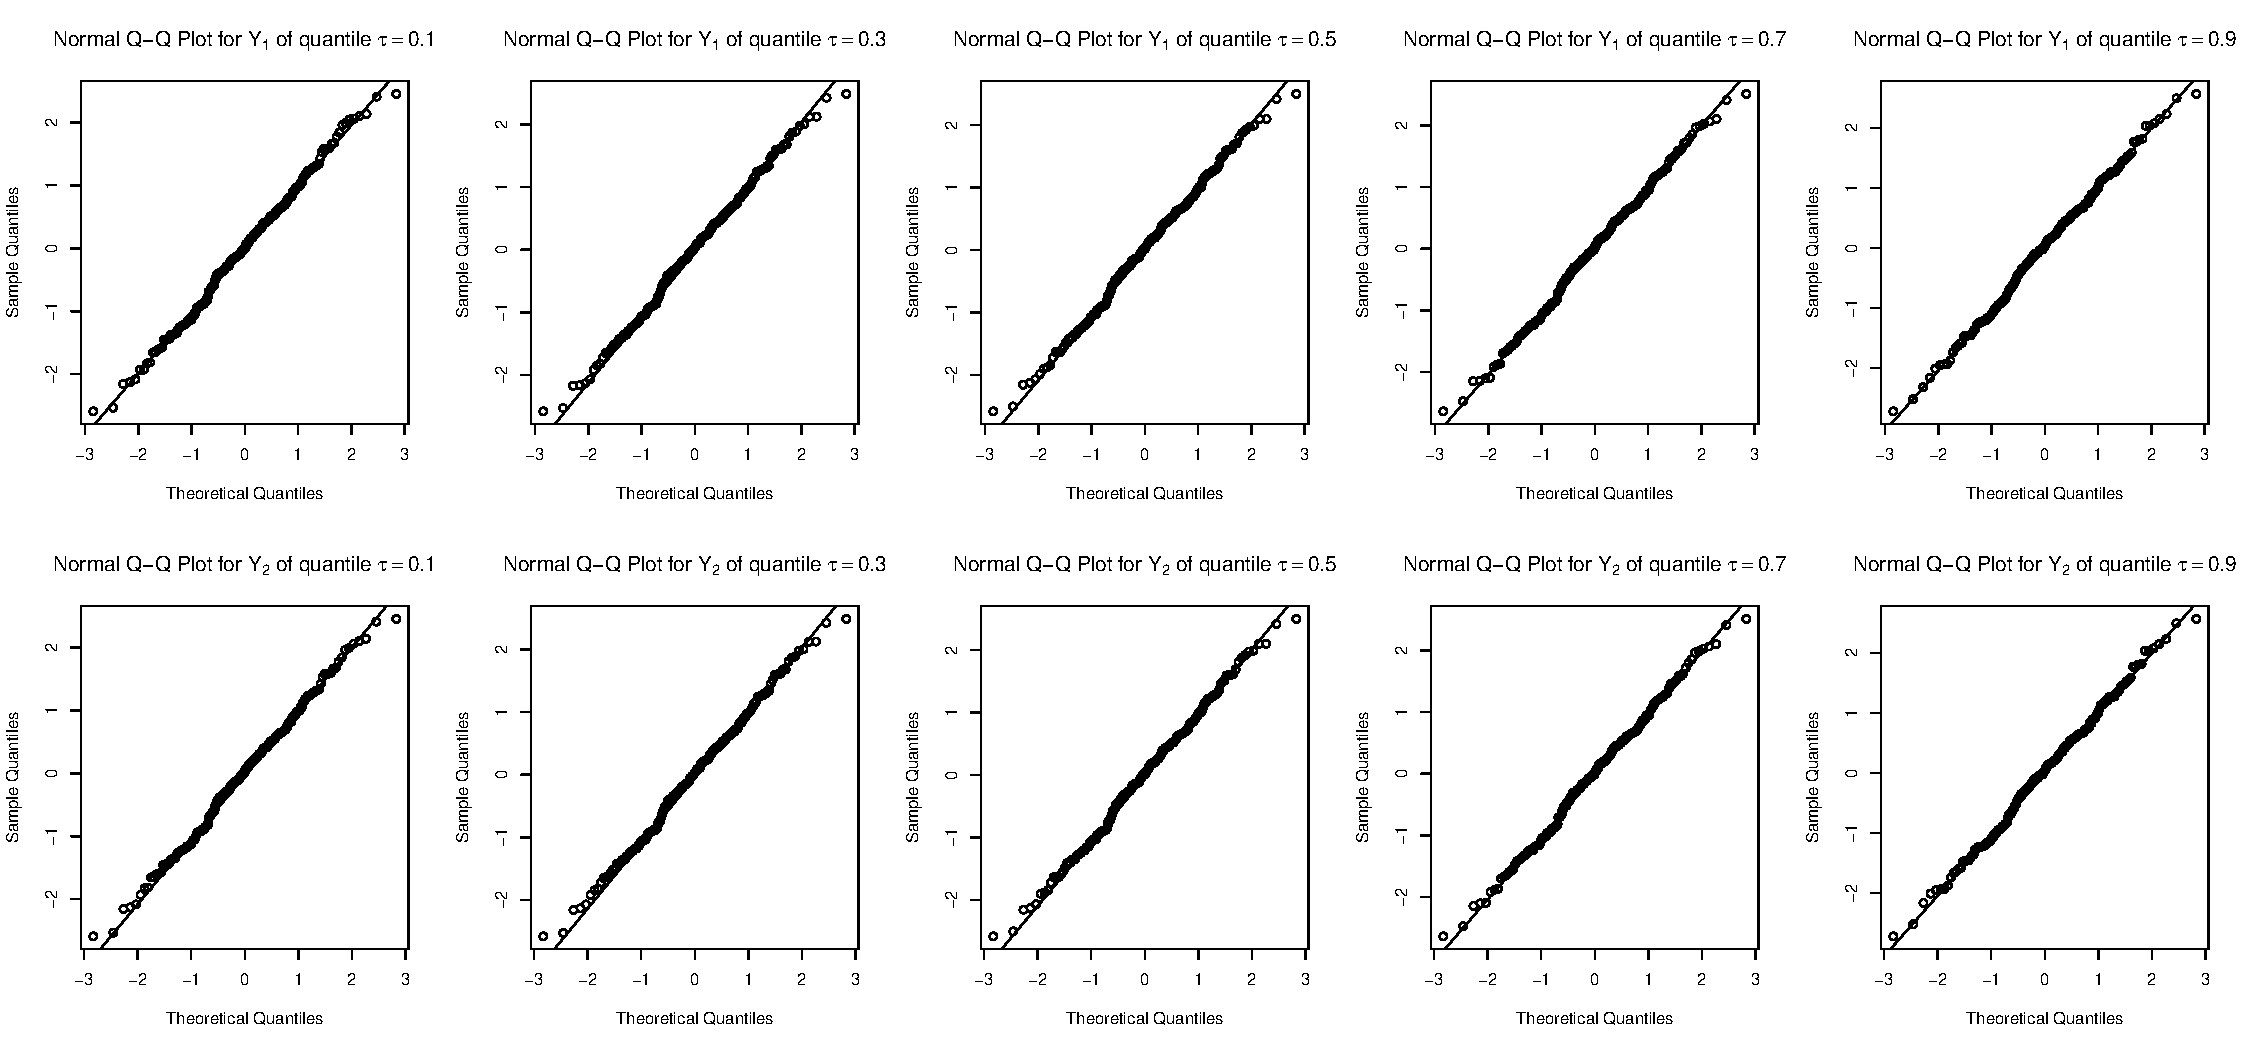
\includegraphics[scale = .4]{../image/ToursGoF}
\label{lastpage}

\end{document}

%%% Local Variables:
%%% mode: latex
%%% TeX-master: t
%%% End:
